\documentclass[border=5mm]{standalone}
\usepackage{tikz}
\usetikzlibrary{calc, intersections}

\begin{document}
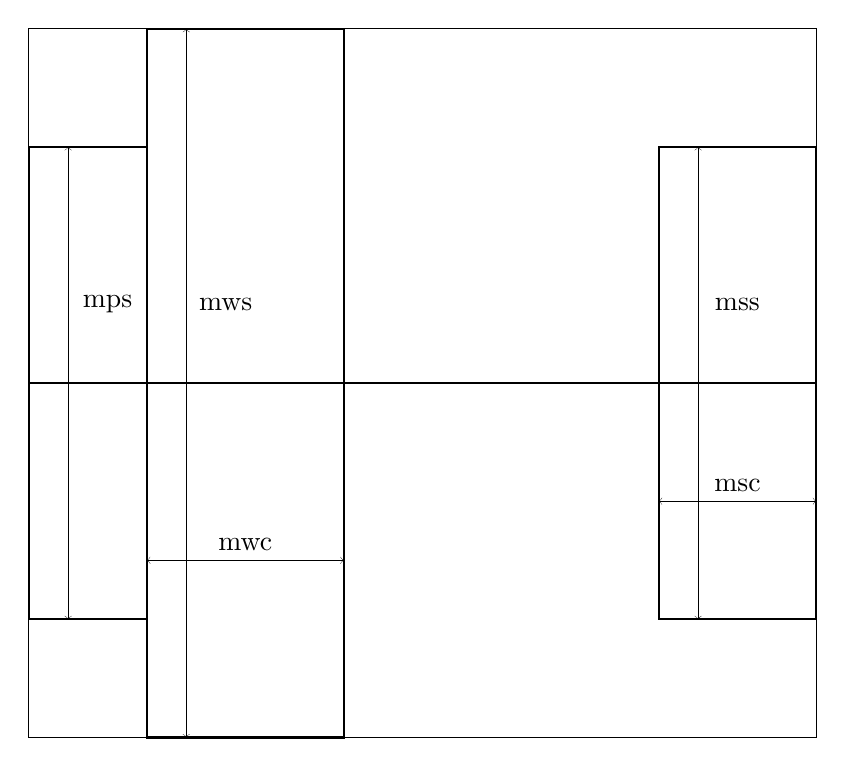
\begin{tikzpicture}

  \coordinate (f0) at (0,0); % name the origin
  \coordinate (f1) at (10,0); % aft end
  \coordinate (w0) at (1.5,4.5);
  \coordinate (w1) at (1.5,-4.5); % left center span
  \coordinate (w2) at (4,-4.5);  % right center
  \coordinate (w3) at (4,4.5);  % right center

  \coordinate (s0) at (8,3);  % right center
  \coordinate (s1) at (8,-3);  % right center
  \coordinate (s2) at (10,-3);  % right center
  \coordinate (s3) at (10,3);  % right center

  \coordinate (p0) at (0,3);  % right center
  \coordinate (p1) at (1.5,3);  % right center
  \coordinate (p2) at (1.5,-3);  % right center
  \coordinate (p3) at (0,-3);  % right center

  \coordinate (b0) at (0,4.5);
  \coordinate (b1) at (10,4.5);
  \coordinate (b2) at (10,-4.5);
  \coordinate (b3) at (0,-4.5);

  % fuselage center line
  \draw[thick] (f0) -- (f1);
  % wing box
  \draw[thick]  (w0) -- (w1) -- (w2) -- (w3) -- cycle;
  % stab box
  \draw[thick]  (s0) -- (s1) -- (s2) -- (s3) -- cycle;
  % prop box
  \draw[thick]  (p0) -- (p1) -- (p2) -- (p3) -- cycle;
  % outer bounding box
  \draw[thin] (b0) -- (b1) -- (b2) -- (b3) -- cycle;

  % wing dimension
  \draw [ultra thin, <->] (1.5,-2.25) -- node [above] {mwc} (4,-2.25);
  \draw [ultra thin,<->] ($(w0) + (0.5,0)$) -- ($(w1) + (0.5,0)$);
  % stab dimension
  \draw [ultra thin, <->] (8,-1.5) -- node [above] {msc} (10,-1.5);
  \draw [ultra thin,<->] ($(s0) + (0.5,0)$) -- ($(s1) + (0.5,0)$);
  % prop dimension
  \draw [ultra thin, <->] (0.5,3) -- (0.5,-3);

  \node at (1,1) {mps};
  \node at (2.5,1) {mws};
  \node at (9,1) {mss};
\end{tikzpicture}
\end{document}
